\chapter{結論}
本論文では

記法メモ\\
Wavenet\cite{oord2016wavenet}は
音声波形を時系列データとして自己回帰モデルで学習することによって,人間の声のような自然な音声を生成することができる.
時点$t$における観測値を$x_t$,$\bm{x} = \left\{ x_1, ..., x_T \right\}$を観測値の全体集合とする.このとき,波形の同時確率は 条件付き確率の積として
以下のよう表現される.
\begin{equation}
	p(\bm{x}) = \prod_{t=1}^T p(x_t | x_1, ..., x_{t-1})
\end{equation}

つまり,$x_t$は前時点の全てにおけるサンプルに条件づけられる.

図\ref{fig:ccl}に因果的畳み込み層のスタックを示す.

\begin{figure}[t]
	\centering
	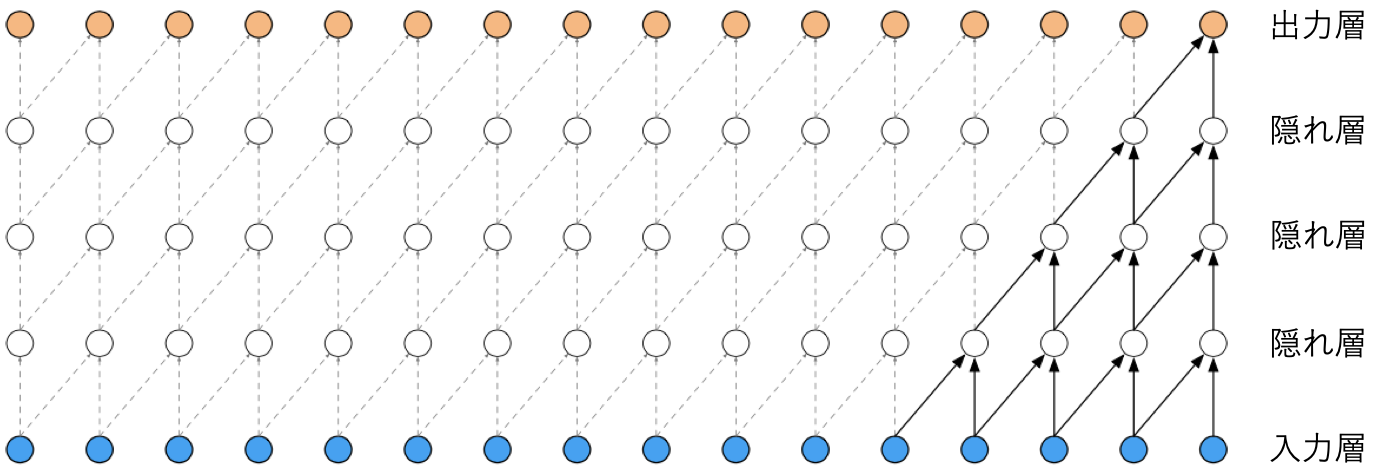
\includegraphics[width=\linewidth]{./figure/ccl.png}
	\caption{因果的畳み込み層}
	\label{fig:ccl}
\end{figure}

\cite{juang1991hidden}は.

今後の課題を以下に挙げる.
\begin{itemize}
	\item の向上
	\par
	必要がある.
	\item への応用
	\par
	を行いたい.
	\newpage
	\item の改善
	\par
	今後,取り組みたい.
\end{itemize}
